\documentclass[11pt]{article}
\usepackage[italian]{babel}
\usepackage[utf8]{inputenc}
\usepackage{graphicx}
\usepackage{float}
\usepackage{amsmath}
\usepackage{amsfonts}
\usepackage{hyperref}
\usepackage{glossaries}
\makeglossaries
\newglossaryentry{magic}{
    name={magic number},
    description={Un magic number è quel numero che metti in una variabile quando è nulla ma non hai il null. Tipo -1}
}
\newglossaryentry{agnostic}{
    name={platform agnostic},
    description={Con platform agnostic intendiamo software che può essere eseguito allo stesso modo su diverse piattaforme}
}
\newglossaryentry{case}{
    name={CASE tool},
    description={Il CASE tool è un software che supporta la progettazione di sistemi software, ad esempio con UML}
}
\newglossaryentry{constraint}{
    name={constraint},
    description={un constraint è un limite che viene posto; restriction, limitation.}
}
\usepackage[normalem]{ulem}
\newcommand{\code}[1]{\texttt{#1}}
\newcommand{\numpy}{{\tt numpy}}    % tt font for numpy
\topmargin -.5in
\textheight 9in
\oddsidemargin -.25in
\evensidemargin -.25in
\textwidth 7in
\begin{document}

% ========== Edit your name here
\author{Simone Montali\\monta.li}
\title{Riassunti di Ingegneria del Software}

\maketitle

\medskip
\section*{Prefazione}
Questo progetto nasce dalla necessità di trovare un metodo di studio per questa materia che, ai più sembra banale. Il problema di fondo è proprio in questa apparente banalità: si finisce per studiarla di fretta pensando di conoscerla, e ci si rende conto troppo tardi di non essere pronti. Mi scuso, anzitutto, per il vocabolario misto italiano-inglese che utilizzerò in queste pagine. Tanti di voi sanno quanto sia complicato esprimere certi concetti in italiano. Ho inserito un piccolo glossario a fine documento. Questo documento ha lo scopo di essere il giusto mezzo tra completezza e sinteticità. Mi scuso, in secundis, per i toni a volte scurrili. Un vero informatico è arrabbiato \textit{/per il codice che non compila/\LaTeX  che fa ciò che vuole/il computer che si impalla/quel piccolo bugfix di Linux che diventa un bagno di sangue/}, e non c'è modo migliore di sfogare le incazzature informatiche che imprecare in riassunti che leggeranno le generazioni a venire. 
Non so come tu ti sia procurato questo documento, ma se hai 5 minuti da buttare, dai una letta alle cose che ho scritto \href{https://monta.li/appunti}{qui.} Ci troverai anche un'altra valangata di appunti. Buona studiata ed in bocca al lupo per tutto.
\section{J1 - Java Overview}
Java è un linguaggio object-oriented, derivato da C/C++, nato per applicazioni web. È semplice, multi-threaded, dinamico. Ha ereditato da C++ la sintassi, la mancanza di puntatori, la garbage collection, la mancanza di header files e preprocessori. Rispetto a C++, però, si avvia più velocemente, richiede meno codice, è indipendente dalla piattaforma e più facile da distribuire. Esistono 3 versioni:
\begin{itemize}
    \item Java Standard Edition (J2SE): applicazioni stand-alone client-side
    \item Java Enterprise Edition (J2EE): applicazioni server-side
    \item Java Micro Edition (J2ME): utilizzato per dispositivi piccoli, come i cellulari
\end{itemize}
Il software viene eseguito sulla \textbf{Java Virtual Machine}, che permette di essere indipendente dalla piattaforma. I file .java contengono i sorgenti, i file .class il codice compilato (\textit{bytecode}). Un file jar contiene il bytecode e i file multimediali, e viene utilizzato per distribuire l'applicazione. 
\subsection{Serializzazione e riflessione}
La serializzazione è il meccanismo che converte oggetti in \textbf{byte streams}. La deserializzazione è il processo inverso. Questo meccanismo è utilizzato per trasferire e salvare oggetti. La \textbf{riflessione} permette a un programma di analizzarsi e manipolare le sue proprietà interne.
\subsection{JRE e JDK}
Il \textbf{Java Runtime Environment} è un pacchetto software contenente la JVM, alcuni librerie (.jar) e altri componenti. Il suo scopo è eseguire applicazioni scritte in Java. Il \textbf{Java Development Kit} è un superset, contenente gli strumenti atti a sviluppare, debuggare e monitorare le applicazioni. 
\subsection{Platform Module System}
Introdotto da Java9, aggiunge un livello di aggregazione oltre ai pacchetti: i \textbf{moduli}. Un modulo definisce un gruppo riutilizzabile di pacchetti e risorse (immagini/XML/...). Un modulo ha bisogno di \textit{Java Module Descriptor}, module-info.java, contenuto nella root del modulo. Può anche dipendere da altri moduli, ma aciclicamente.
Le sue caratteristiche principali sono:
\begin{itemize}
    \item Configurazione affidabile: la modularità permette di dichiarare con chiarezza le dipendenze
    \item Forte incapsulamento: i pacchetti in un modulo sono accessibili solo se esportati
    \item Piattaforma Java scalabile: la piattaforma java include tanti moduli, ma si può creare dei custom runtime per caricare solo i moduli necessari
\end{itemize} 
Il \textbf{module descriptor} include nome, dipendenze, pacchetti esportati, servizi forniti, servizi utilizzati, e una lista dei moduli che sfruttano la reflection.
\subsection{Garbage collector}
Il \textbf{garbage collector} controlla la memoria e trova quali oggetti non sono più "referenziati" da variabili, per eliminarli. Inoltre, compatta gli oggetti rimanenti. Il GC non può essere invocato esplicitamente, ma si può suggerire alla JVM di farlo girare.
\section{J2 - Development tools}
\begin{itemize}
    \item \textbf{Eclipse} è l'IDE che va per la maggiore su Java. È una piattaforma aperta, espandibile con plugin, che fornisce tool per programmare, compilare, debuggare. 
    \item \textbf{Papyrus} è un editor UML basato su Eclipse, fortemente incentrato sulla customizability. Supporta anche i constraint OCL (vedi T12).
\end{itemize}
\subsection{Build tools}
I \textbf{build tools} vengono utilizzati per compilare e costruire immagini software dal source code. Richiedono due componenti: un build script che definisce le task da eseguire, ed un eseguibile che lo processa. Gli script dovrebbero essere \gls{agnostic}.
\subsubsection{Maven}
\textbf{Maven} è un tool di software project management che fornisce un setup di progeto semplice, con dipendenze e management di release e distribuzione. Incoraggia l'uso di una repository centrale di JAR e dipendenze. Permette la scrittura di plugin. I build files sono scritti in XML utilizzando il formato \textit{Project Object Model} (POM), i pom.xml.
\subsection{Static Analysis Tools}
Questi tool possono trovare bug ispezionando il codice senza eseguirlo. Alcuni esempi sono Checkstyle, PMD, SpotBugs. Si overlappano in parte, ma si distinguono tra loro. Idealmente, andrebbero usati tutti. 
\begin{itemize}
    \item \textbf{Checkstyle} permette di seguire un coding standard, automatizzando il processo di verifica. Ha dei file di configurazione in XML.
    \item \textbf{PMD} utilizza un set di regole che analizzano diversi fattori del codice, come codice inutilizzato, duplicato, \textit{over-complicato}
    \item  \textbf{SpotBugs} verifica un set di bug patterns, come null pointers, cicli infiniti, deadlocks...
\end{itemize}
\subsection{Altri tool}
\subsubsection{VisualVM}
VisualVM è un tool che integra dei tool da linea di comando di JDK. Monitora l'utilizzo della CPU, del GC, di memoria, thread e classi caricate. Fornisce inoltre informazioni sui crash. Può venire utilizzato sia in production che development.
\subsubsection{JUnit}
\textbf{JUnit} è un software open source per lo unit testing di Java. Fornisce supporto per la scrittura, l'esecuzione e le annotazioni dei test. Fornisce assertion per verificare i risultati. 
\subsubsection{Mockito}
\textbf{Mockito} è un tool open source per il mocking e lo unit testing. Supporta la creazione di oggetti simulati che simulano oggetti reali in modalità controllate. Offre una sintassi semplice e leggibile, con annotazioni necessarie a ridurre il boilerplate. 
\section{J3 - Using Maven and formatting code}
Il build con Maven segue un life cycle specifico per deployare e distribuire il progetto. Di default, abbiamo tre life cycles:
\begin{itemize}
    \item Default: ciclo principale, deploya il progetto
    \item Clean: Pulisce il progetto e rimuove i file generati dal build precedente
    \item Site: genera la documentazione
\end{itemize}
Ogni life cycle consiste in una serie di fasi. 
Le fasi più importanti:
\begin{itemize}
    \item \textbf{Validate} controlla che tutte le informazioni necessarie siano presenti
    \item \textbf{Compile} compila il codice
    \item \textbf{Test-compile} compila il codice di test
    \item \textbf{Test} esegue gli unit tests
    \item \textbf{Package} builda un pacchetto distribuibile (jar,war,...)
    \item \textbf{Integration-test} esegue gli integration tests
    \item \textbf{Install} installa il pacchetto in una repo locale
    \item \textbf{Deploy} copia il pacchetto sulla repo remota
\end{itemize}
I \textbf{plugins} sono utilizzati per inserire altri goal nella build phase. I build plugins sono eseguiti nella build phase, mentre i reporting nella reporting phase. Tutti i plugin devono avere informazioni di base come \textbf{groupID}, \textbf{artifactId}, \textbf{version}.
Le \textbf{dipendenze} aiutano a definire, creare e mantenere delle build stabili con class-path e versioni definite. Possono caricare file jar dalle repositories, che conservano artifatti e dipendenze varie. Le repositories possono essere locali o remote. Maven, di default, usa la \textbf{central Maven repository.}
I \textbf{profili} modificano il POM a build time, definendo una serie di modifiche da fare al POM quando attivati. Ad esempio, se avessimo un DB staging e uno di produzione.
\section{J4 - Language structures}
Elenchiamo ora alcune linee guida per la programmazione:
\begin{itemize}
    \item Preferire l'utilizzo dei for-each o degli iteratori, piuttosto che indici, che inducono in errore
    \item Utilizzare array di lunghezza nulla per rappresentare il null
    \item Con \textbf{widening} intendiamo il casting di un subtype al suo genitore. Esso è svolto automaticamente durante un assegnamento. 
    \item Con \textbf{narrowing} intendiamo il casting di un supertype a un suo figlio. Questo richiede un casting esplicito per colpa dello strong typing di Java.
\end{itemize}
\section{J5 - Packages, classes, interfaces}
Un \textbf{package} fornisce un namespace logico per un gruppo di classi \textit{related}. I pacchetti definiscono una struttura descritta da un directory tree. Ogni pacchetto è descritto dal suo \code{package-info.java}, che deve essere nella directory. 
\subsection{Classes}
Una \textbf{classe} è un'entità logica che definisce un gruppo di oggetti aventi attributi e metodi comuni. Alcune convenzioni di naming:
\begin{itemize}
    \item Utilizzare nomi inglesi
    \item Utilizzare il mixed case (es. volevoMettereUnaBestemmia)
    \item Usare poche abbreviazioni e con consistenza
    \item Usare le parole complete al posto di acronimi (no: PD)
    \item Usare terminologia specifica
    \item Evitare nomi lunghi
    \item Evitare caratteri speciali all'inizio e alla fine
    \item Evitare nomi da una lettera (@Guido parlo a te, ti tengo d'occhio)
    \item Le classi devono avere l'iniziale maiuscola, il resto no
    \item Le costanti essere maiuscole con underscore a separare le parole
    \item I pacchetti dovrebbero essere minuscoli, separati da punti 
    \item Il prefisso di un pacchetto è solitamente il sito web dell'organizzazione
\end{itemize}
La keyword \textbf{this} è utilizzata per accedere a metodi e attributi della classe in uso. La keyword \textbf{super} è utilizzata per accedere a metodi della superclasse. Non possono ovviamente essere usati in metodi statici. \textit{Se non è così ovvio suggerirei un ripassino.} Queste keyword si possono usare anche per chiamare costruttori. Una classe può accedere ad un'altra tramite il nome, se è nello stesso pacchetto, o utilizzando il \textit{qualified name} se è in un altro. Si può anche importare classi da un pacchetto.
\subsubsection{Incapsulamento}
L'\textbf{incapsulamento} è una forma di protezione; il mondo esterno non ha accesso all'implementazione interna dell'oggetto. I dati vengono nascosti, e si ottiene l'accesso solo tramite metodi: questo ne assicura l'integrità. Per l'incapsulamento sono fondamentali i visibility modifiers. 
\begin{figure}[H]
    \centering
    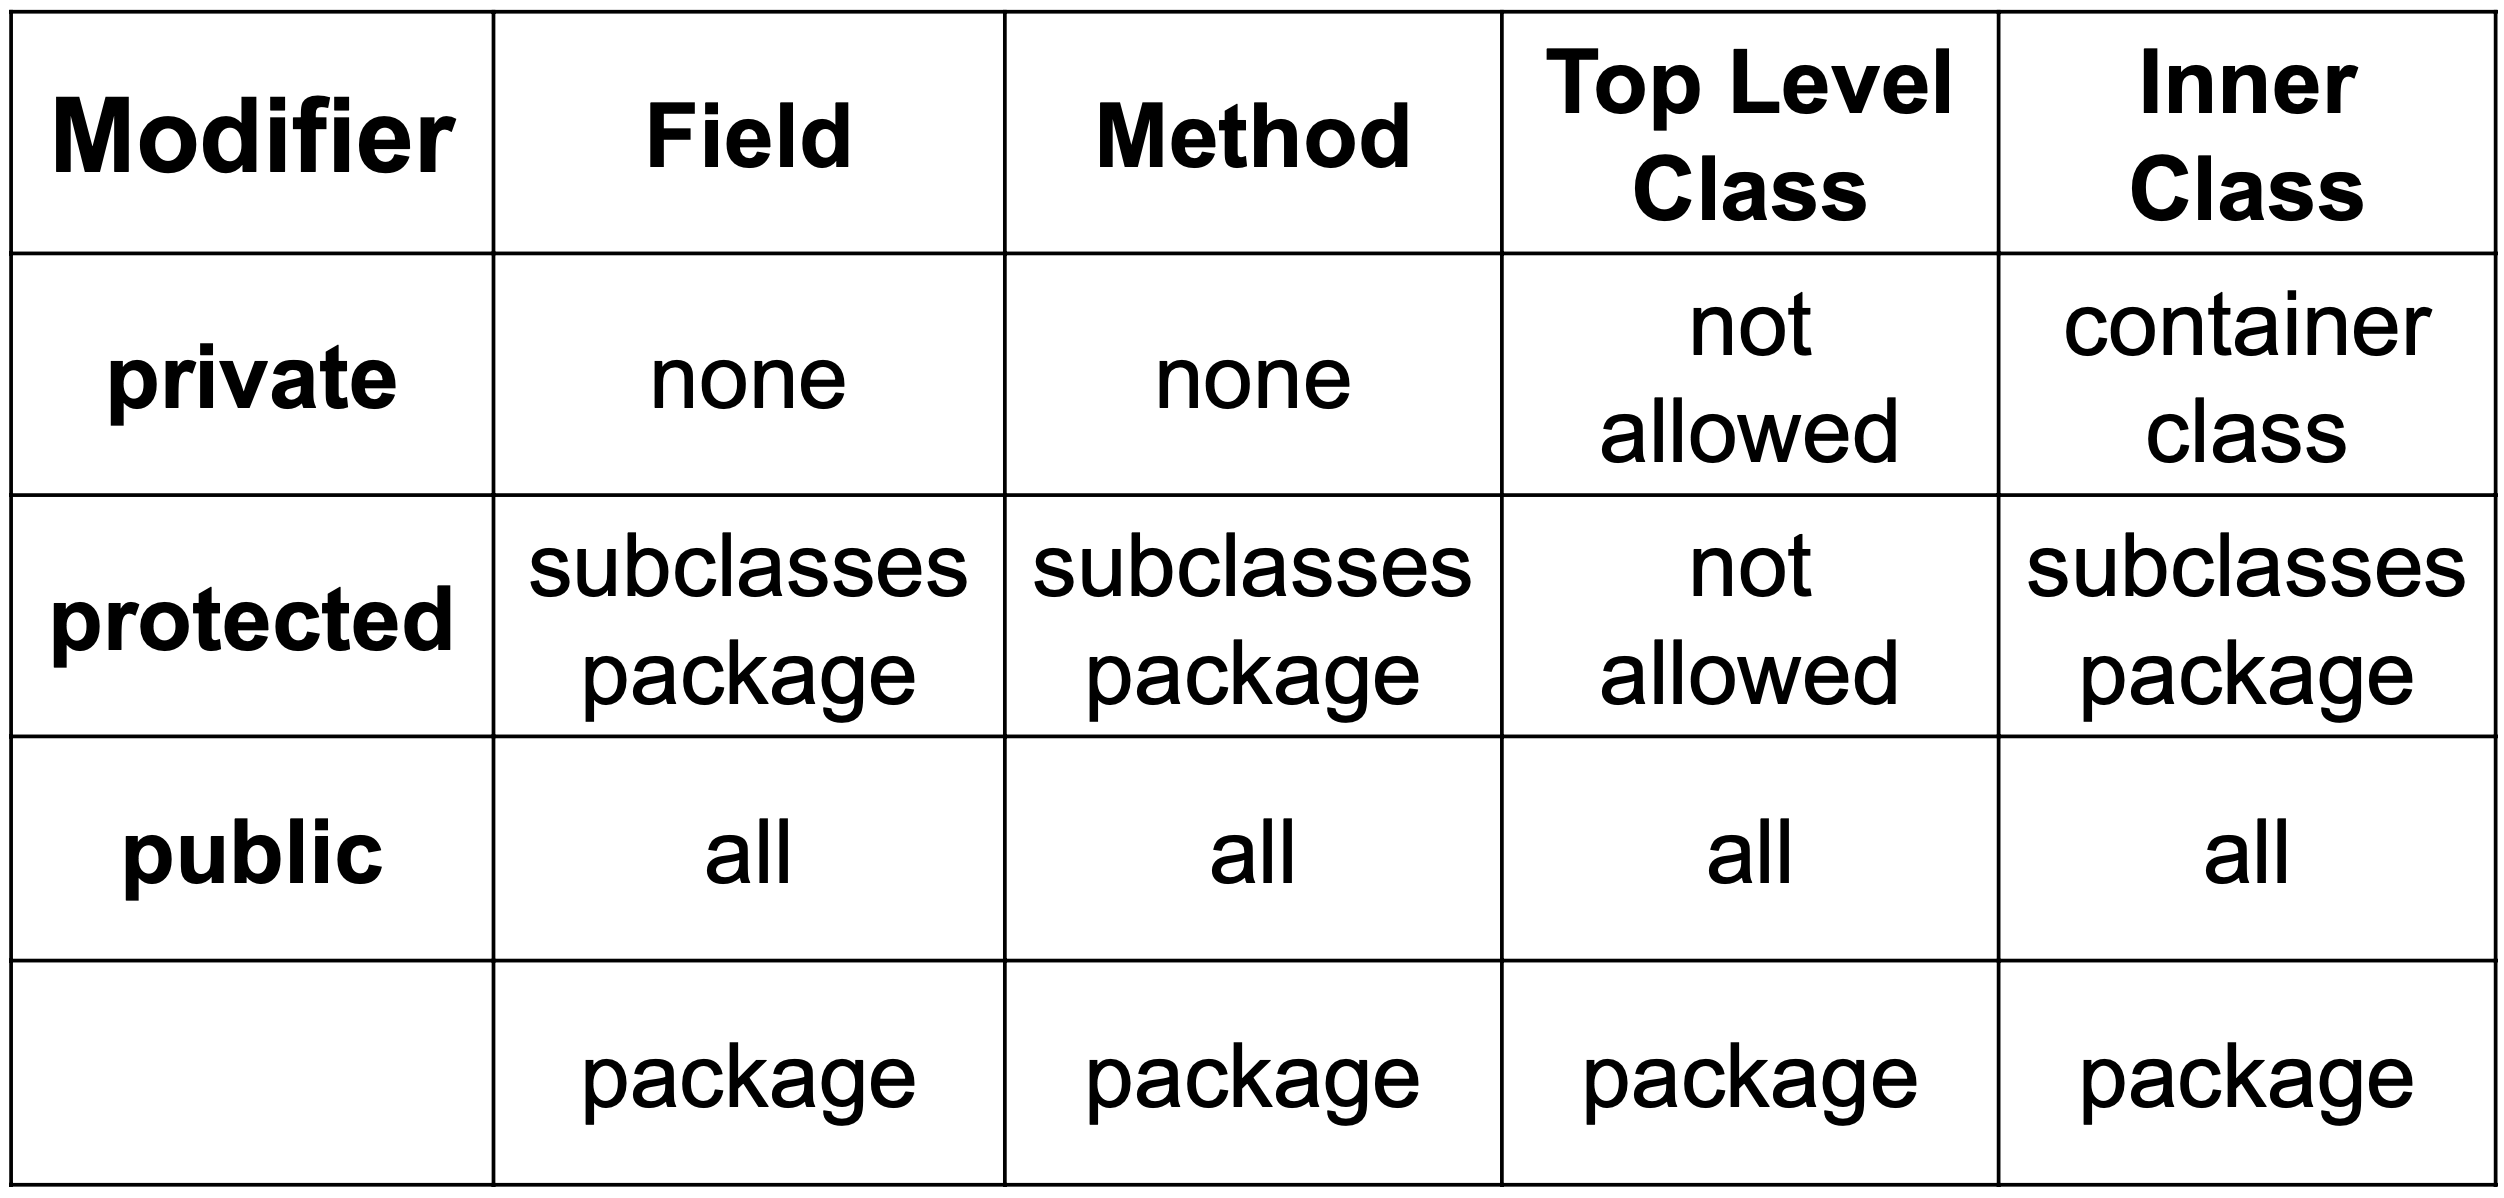
\includegraphics[width=0.6\linewidth]{res/java/VisibilityModifiers.png}
    \caption{Modificatori della visibilità}
\end{figure}
\subsubsection{Methods}
I metodi sono delle funzioni che eseguono determinate operazioni, permettendo il riutilizzo del codice. Accettano parametri e ne restituiscono altri.
I \textbf{costruttori} sono metodi speciali che creano istanze di classe. Una classe può avere piò costruttori. Il nome è quello della classe. Se non sono definiti costruttori, viene utilizzato quello di default (vuoto), che viene invocato anche dalle subclasses.
Alcune convenzioni per i metodi:
\begin{itemize}
    \item Validare gli argomenti prima di utilizzarli: \textit{mai dare per scontato che l'utente non sia una scimmietta incazzata.}
    \item Utilizzare la keyword \code{final} per gli argomenti, in modo da non poterli modificare nel codice
    \item Spaziare gli argomenti nella lista. \textit{Ma non fate le bestie di satana mettendo lo spazio dopo la parentesi}
\end{itemize} 
\subsubsection{Fields and variables}
Le variabili forniscono spazio in memoria. Hanno un tipo specifico che determina la memoria occupata, i valori assumibili, le operazioni applicabili. Il loro scope dipende dal modifier associato. \textbf{Lo scope delle variabili locali inizia nel punto di dichiarazione e finisce con la fine del blocco dove sono state dichiarate.} A partire da Java10, in alcuni casi non è necessario dichiarare il tipo. \textit{/s Am I PHP-dreaming?}
\subsection{Static fields, methods, blocks}
Gli attributi/metodi statici esistono indipendentemente dagli oggetti. Possono quindi essere chiamati senza presenza di oggetti, ma con alcune restrizioni: possono chiamare solo metodi statici, possono accedere solo a campi statici, non possono usare this/super. Sono ovviamente condivisi tra tutte le istanze. Un blocco static viene caricato una sola volta quando una classe viene caricata. 
\subsection{Final classes, methods, fields}
Una classe dichiarata \code{final} non può essere estesa. Un metodo \code{final} non può essere overridato. Un field \code{final} non può essere modificato, è quindi costante. Va inizializzato alla dichiarazione, nei costruttori o in un blocco static. 
\subsection{Classe Serializable}
Una classe che implementa l'interfaccia \code{Serializable} deve rispettare uno di questi tre constraints:
\begin{itemize}
    \item Contenere dati primitivi
    \item Contenere oggetti Serializable
    \item Essere un transient 
\end{itemize}
\subsection{Oggetti immutabili}
I campi sono final, le subclasses non possono overridare metodi. I metodi non possono modificare gli oggetti mutabili collegati ai fields, in quanto non sono condivisi. 
\subsection{Coding Conventions}
Elenchiamo ora qualche coding convention.
\subsubsection{Field coding conventions}
\begin{itemize}
    \item Dichiarare i campi private per fornire incapsulamento
    \item Inizializzare i final all'interno dei costruttori
    \item Non inizializzare i campi numerici con \glspl{magic}, ma usare una costante
\end{itemize}
\subsubsection{Variable coding conventions}
\begin{itemize}
    \item Dichiarare le variabili appena prima del loro utilizzo
    \item Evitare l'assegnamento di più variabili allo stesso valore in un singolo statement
    \item Non utilizzare i \glspl{magic}
    \item Separare i membri in base al loro scope 
    \item Utilizzare nomi esplicativi
\end{itemize}
\subsubsection{JavaBean classes coding conventions}
\begin{itemize}
    \item Dovrebbero avere un costruttore vuoto
    \item Dovrebbero essere Serializable $\rightarrow$ supporta uno storing/restoring affidabile delle istanze 
    \item Dovrebbe avere getter/setter con una convenzione di nomi: getCampo, setCampo, o se boolean anche isCampo
\end{itemize}
\subsection{Ereditarietà}
L'ereditarietà è il meccanismo che permette di ereditare campi e metodi delle superclassi. Il vantaggio principale è il riutilizzo del codice. Le subclasses non possono usare i campi privati, ovviamente. Possono anche overridare i metodi non final. 
\subsection{Method overloading e overriding}
L'overloading avviene quando abbiamo più implementazioni dello stesso metodo, cambiando gli argomenti ma avendo ugual nome e return type. Un metodo è overridden quando una subclass ridefinisce un metodo con la stessa firma della classe padre. 
\subsection{Abstract classes}
Le classi astratte forniscono un'implementazione parziale

\printglossary

\end{document}